\section{Methodology}
\label{sec:method}

%%----------------------------------------------------------------
%% Overview Figure
%%----------------------------------------------------------------
\begin{figure*}[t]
	\begin{center}
	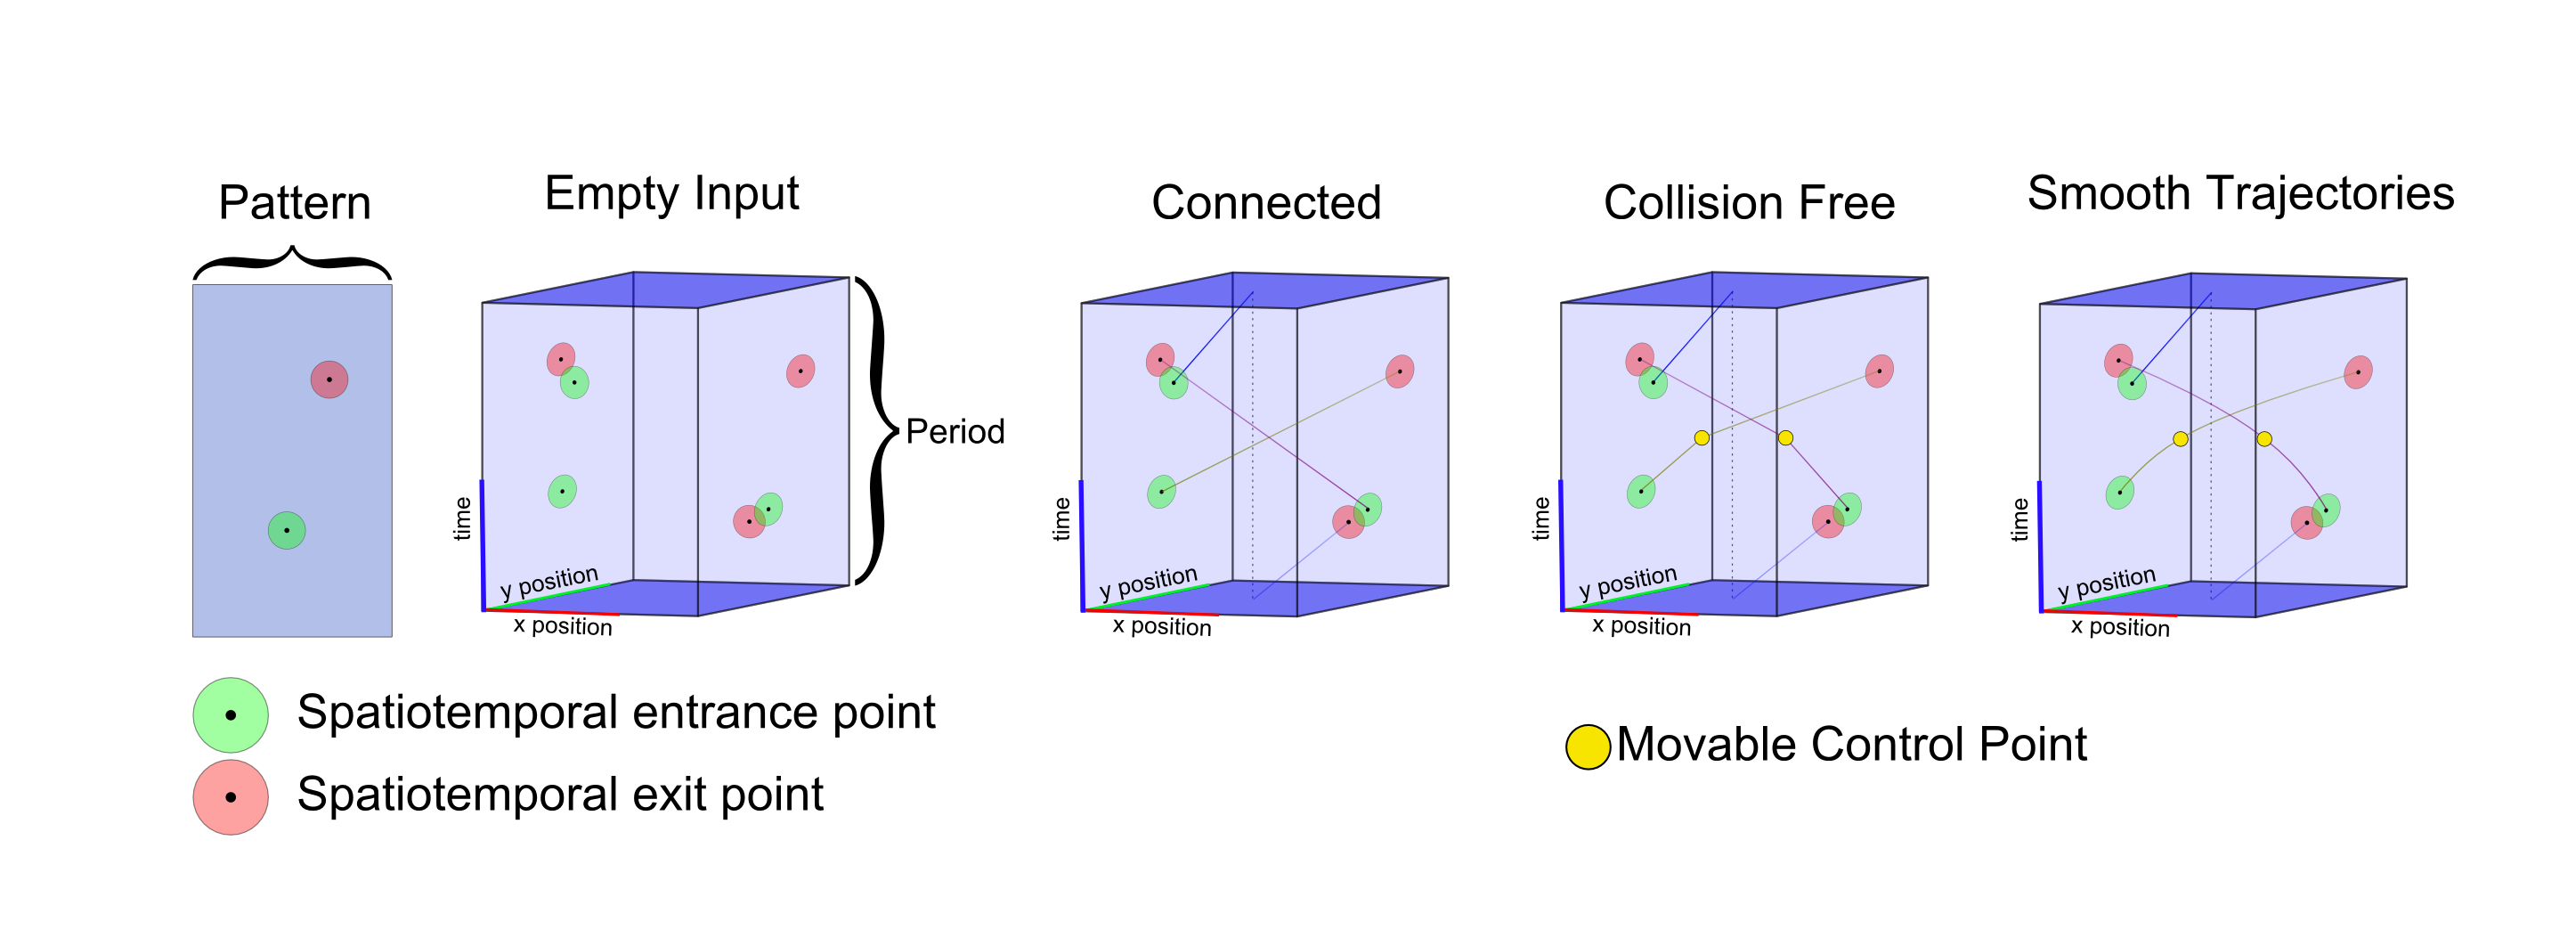
\includegraphics[width=0.9\linewidth]{./images/overview-hd-old.png}
% 	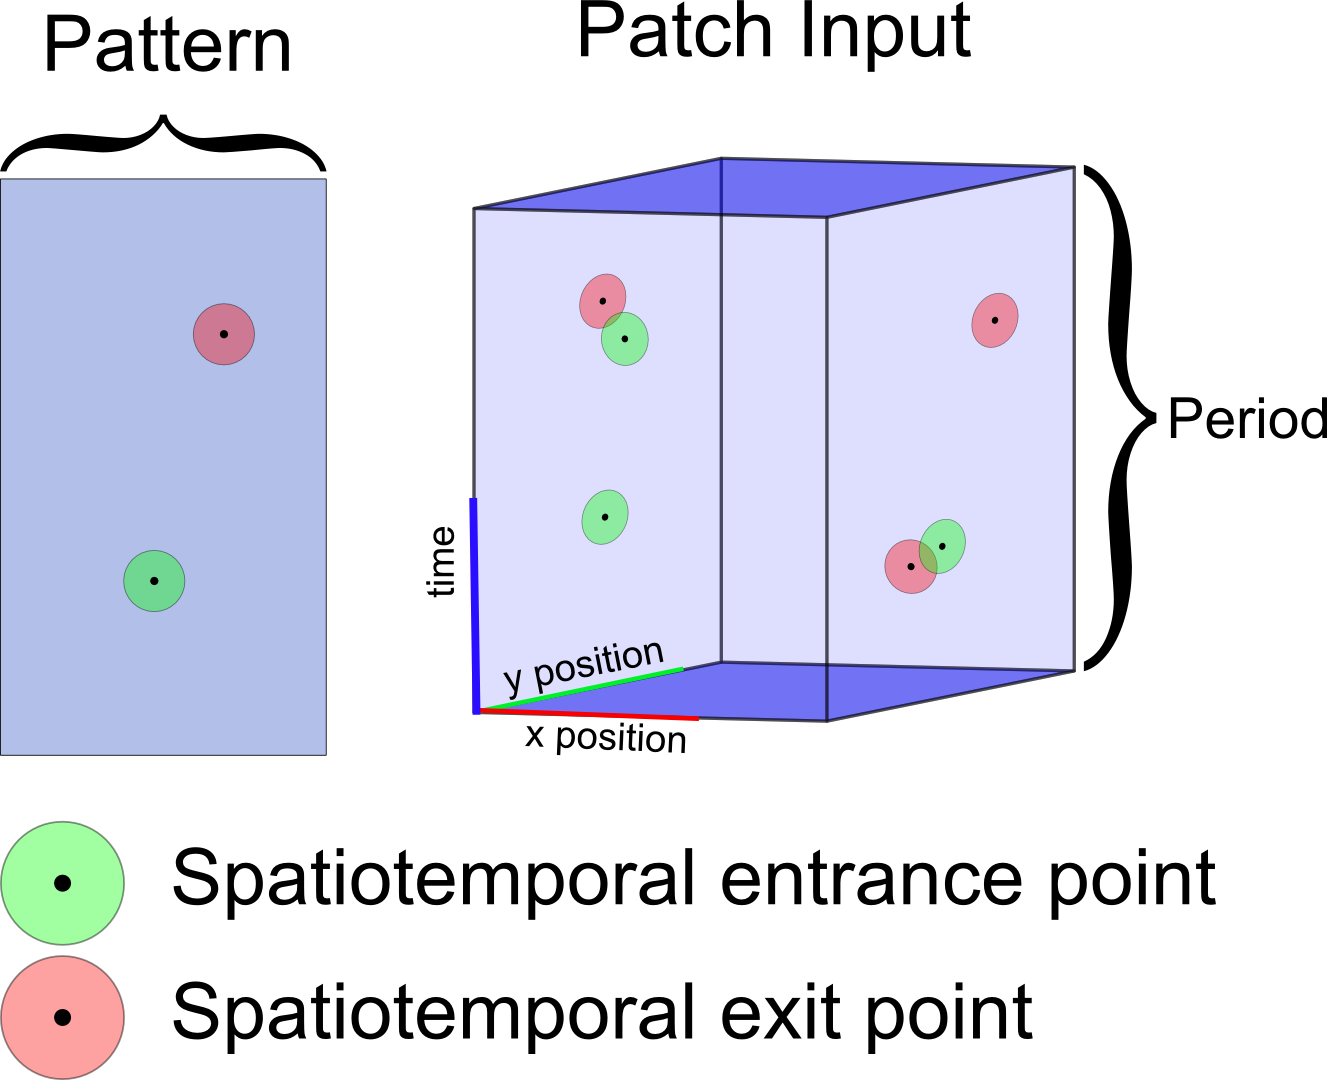
\includegraphics[height=4cm]{./images/patches-empty-patch-with-pattern.png}
% 	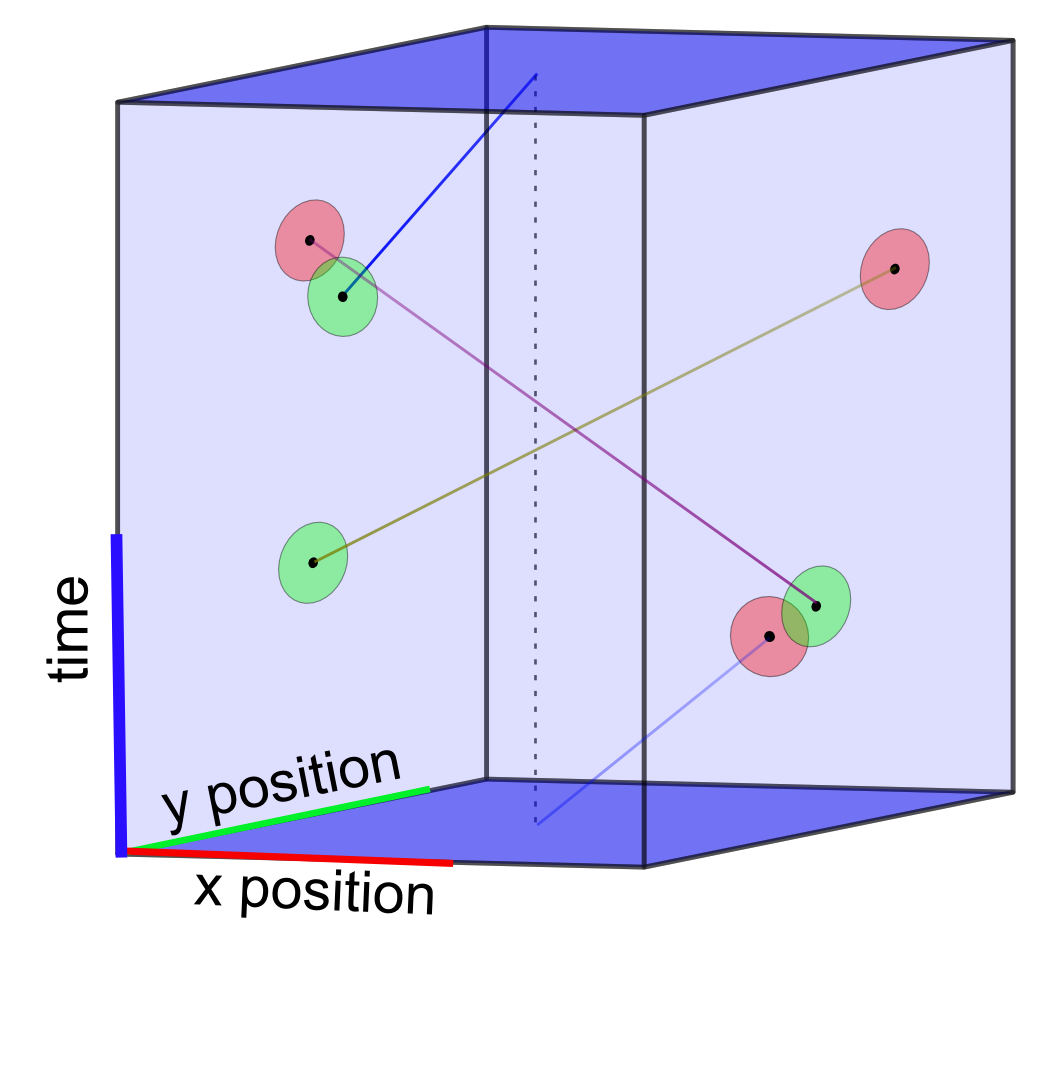
\includegraphics[height=4cm]{./images/patches-connected-patch.png}
% 	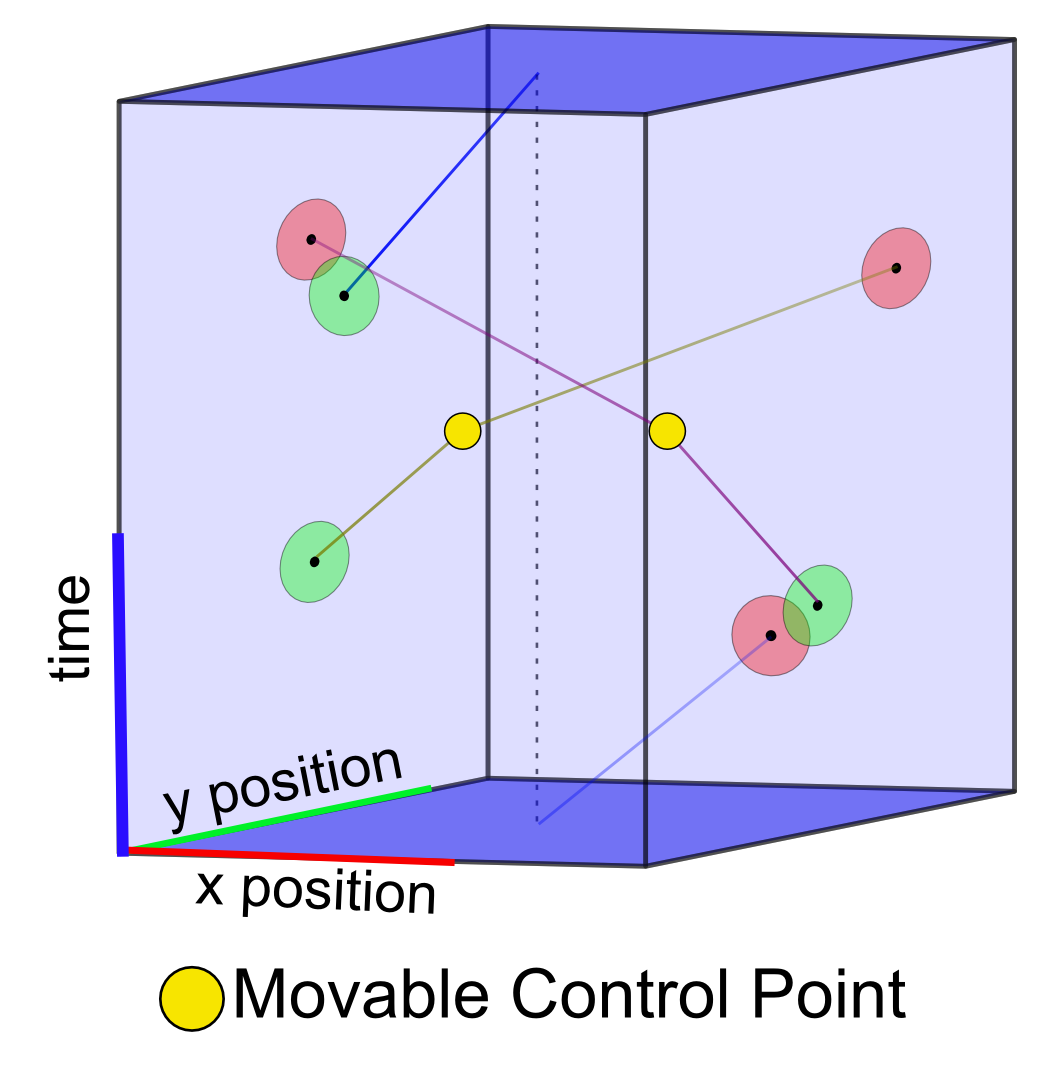
\includegraphics[height=4cm]{./images/patches-collision-free-patch.png}
% 	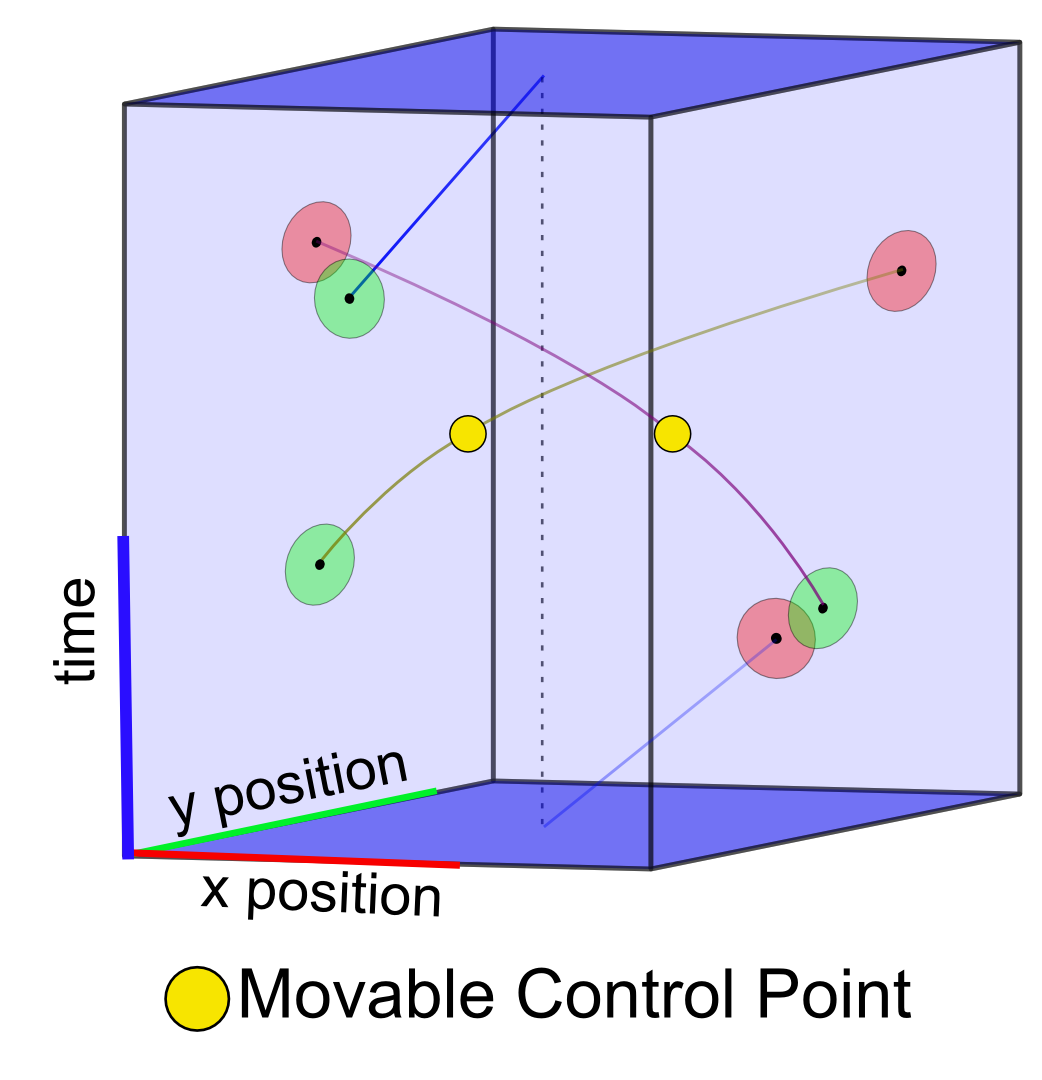
\includegraphics[height=4cm]{./images/patches-smoothed-patch.png}
	\caption{
		\textbf{Overview} Input and output points in a patch's patterns are initially connected and subsequently modified using the proposed optimization approach and smoothed out to be collision free.
	}
	\label{fig:overview}
	\end{center}
\end{figure*}
%%----------------------------------------------------------------
%% Overview Figure
%%----------------------------------------------------------------

%\note{Overview: remind definitions on crowd patches: patch, pattern, spatiotemporal waypoints (boundary conditions: input, output, initial states // boundary conditions should be strictly enforced. Movable control points), period of time \dots}

In this section we present the proposed methodology for generating trajectories for patches.
We first give some definitions and notations (Section~\ref{sec:method:definitions}), followed by an overview of the method (Section~\ref{sec:method:overview}), and trajectories initial generation, collision handling and smoothing out (Sections~\ref{sec:method:init}--\ref{sec:method:smoothing}).

%%===============================================================
%% Subsection: Patch Definitions
%%===============================================================
\subsection{Definitions}
\label{sec:method:definitions}

Before presenting our approach on trajectory generation for Crowd Patches, we present some definitions and notations regarding Crowd Patches.
Please refer to Figure~\ref{fig:definitions} for a visual representation of the definitions and \cite{Yersin:2009} for a more detailed description.

%%----------------------------------------------------------------
%% Patch Definitions
%%----------------------------------------------------------------
\begin{figure}
\begin{center}
	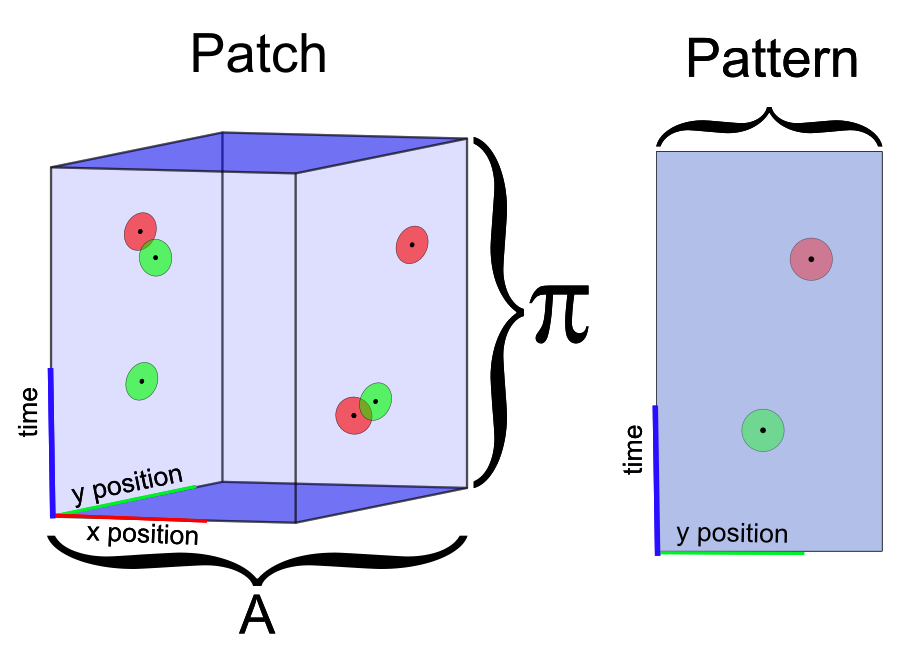
\includegraphics[width=0.9\linewidth]{./images/patch-definitions.png}
	\caption{
		\textbf{Patches and Patterns} A \emph{patch} is defined by the geometrical area $A$ where a set of dynamic and static objects ($D$ and $S$ respectively) can move over a period of time $\pi$. \emph{Patterns} define boundary conditions for the patches and act as portals connecting neighboring patches. 
	}
	\label{fig:definitions}
	\end{center}
\end{figure}
%%----------------------------------------------------------------
%% Patch Definitions
%%----------------------------------------------------------------
 
%\begin{description}

%\item[Patch]{
A \textbf{patch} is a set $\{ A, \pi, D, S\}$ where $A$ is geometrical area with a convex polygonal shape, $\pi$ the period of time of the animation and $D$ and $S$ are the sets of dynamic and static objects, respectively. 
These last two sets may be empty in case of an empty patch.
%This implies that objects in sets $D$ and $S$ move in the area defined by $A$ over some period in time $[t_1, t_2]: 0\le t_1 < t_2 \le \pi$. 
%}

%\item[Static obstacles]{
\textbf{Static objects} are simple obstacles whose geometry is fully contained inside the patch.
%}

%\item[Dynamic objects]{
\textbf{Dynamic objects} are animated; i.e., they are moving in time according to a set of trajectories $T$.
%}

%\end{description}

\subsubsection{Trajectories}

We define a {\bf trajectory} inside a patch as a function $\tau(t)$ going from time to position, more specifically from a subset of $[ 0,\pi ]$ to $A$:

\begin{equation}
	\tau:[t_1,t_2]\rightarrow A, \hspace{0.3cm} 0 \leq t_1 < t_2 \leq \pi
	\label{eqn:trajectory}
\end{equation}

We represent a trajectory as a list of control points connected by segments:

\begin{itemize}
  \item A {\bf control point} is a point in space and time $\mathbf{cp} = \{\mathbf{p}_{cp}, t_{cp}\}$.
All control points in a trajectory can either be boundary or movable ones.
Boundary control points serve as entry and exit points to the patch and cannot be moved, added or deleted.
Movable control points on the other hand can be moved, added, or removed from the trajectory as long as they do not violate the constraints of the patch; i.e., their positions must lie inside area $A$~($\mathbf{p}_{cp} \in \mathbf{A}$) and their time $t_{cp}$ must be between $t_1$ and $t_2$.
 \item A {\bf segment} is a straight line connecting two control points in a specific order. Since these are unidirectional lines in space-time, it is important to remember that they are not allowed to go backwards in time.  
\end{itemize}


There are two categories of dynamic objects: endogenous and exogenous agents.
{\bf Endogenous agents} remain inside $A$ for the total period of time $\pi$.
In order to achieve periodicity for the animation, they are associated with a trajectory $\tau : [0,\pi] \rightarrow A$, such that it respects the periodicity condition: the position at the start and at the end of the animation must be the same, i.e. \mbox{$\tau (0) = \tau (\pi)$}.

{\bf Exogenous agents} on the other hand go outside $A$.
They enter the patch at time $t_{initial}$ and position $\mathbf{p}_{initial}$, and they exit at time $t_{final}$ and position $\mathbf{p}_{final}$.
For each agent we associate a sequence of $n \ge 1$ trajectories $\{ \tau_1, \tau_2, \dots, \tau_n\}$.
Sequences may have only one trajectory, but some agents require additional trajectories in order to satisfy speed and time constraints.
The following conditions must be respected in each sequence of trajectories associated with an exogenous agent:

\begin{enumerate}
	\item $\mathbf{p}_{initial}$ and $\mathbf{p}_{final}$ must be points on the borders of $A$ otherwise they cannot be exogenous agents.
	\item If the sequence is composed by more than one trajectory, for each two contiguous trajectories, the following must be true to ensure continuity: $\tau_i(\pi) = \tau_{i+1}(0)$.

\end{enumerate}

Note that the second condition implicitly implies that in sequences with multiple trajectories, each middle trajectory must be fully defined in the period of time $[0,\pi]$, while $\tau_1$ must be defined in $[t_{initial},\pi]$ and $\tau_n$ must be defined in $[0, t_{final}]$.


\subsubsection{Patterns}

% \begin{description}
% 
% \item[Pattern -]{
A patch can be considered as a spatio-temporal right prism depending on the type of polygon used as its area (cube in the case of a squared area patch).
A \textbf{pattern} can be defined as one lateral side of the prism (Figure~\ref{fig:definitions}).
Specifically, it is a rectangle whose base is one of the edges of the polygonal area (we define $\mathbf{l} \in \mathbb{R}^2$ as this two dimensional vector), and its height is equal to the period $\pi$.
In addition to these, patterns also include the sets $\mathbf{I}$ and $\mathbf{O}$ of input and output boundary control points respectively.
The input set contains the boundary control points where exogenous agents begin their trajectories; we call these \emph{entry points}.
Conversely the elements of output are called Exit Points; they establish the position in time and space that the exogenous agents finish their paths.
Formally defined, a pattern $\mathbf{P}^{(i)}$ is:

\begin{equation}
% 	\mathbf{P}_i = \{\mathbf{l}_i, \pi, I_i [p_i, t_i], O_j[p_j, t_j]\}
	\mathbf{P}^{(i)} = \{\mathbf{l}^{(i)}, \pi^{(i)}, \mathbf{I}^{(i)}, \mathbf{O}^{(i)}\}
\end{equation}

To populate virtual environments, patches are concatenated together.
Thus, continuity between trajectories should be enforced for exogenous agents passing through two contiguous patches.
This means that two adjacent patches must have a similar pattern on the side they share; i.e., the vector $l$ and period $\pi$ must be the same and the input and output sets must be exchanged.
More formally, having two patterns $\mathbf{P}_1$ and $\mathbf{P}_2$ where
$P^{(1)}=\{\mathbf{l}^{(1)}, \pi^{(1)}, \mathbf{I}^{(1)}, \mathbf{O}^{(1)}\}$ and~
$P^{(2)}=\{\mathbf{l}^{(2)}, \pi^{(2)}, \mathbf{I}^{(2)}, \mathbf{O}^{(2)}\}$, then, in order to satisfy $C^0$ continuity the following must apply:

\begin{equation}
	l^{(1)}=l^{(2)}, \pi^{(1)}=\pi^{(2)}, \mathbf{I}^{(1)} = \mathbf{O}^{(2)}, \mathbf{I}^{(2)} = \mathbf{O}^{(1)}
% 	\forall \mathbf{cp}_i \in \mathbf{I}^{(1)} \exists \mathbf{cp}_o \in \mathbf{O}^{(2)}
\end{equation}

Under these conditions, $P_1$ is the mirror pattern of $P_2$ and vice versa.
When these patches are animated, this will be observed as moving agents going from one patch to adjacent ones. 
If the area $\mathbf{A}$ of a patch is a square then 4 patterns are defined, one per side.
Patterns defined by a patch have the property that the sum of the cardinality of all the inputs is the same as the sum of the cardinality of all outputs; we call this the parity condition: $\sum(|inputs|)= \sum(|outputs|)$.

A patch defines a set of patterns, and conversely, a set of patterns satisfying the parity condition, having the same period, and whose vectors define a convex polygonal area, can be used to create a patch indirectly.
%  }
% 
% \end{description}

%%===============================================================
%% Subsection: Method Overview
%%===============================================================
\subsection{Overview}
\label{sec:method:overview}

The objective is, given a set of patterns, we want to construct a patch.
This process has three main steps:
\begin{enumerate}
  \item Make a matching between the elements in the Input and Output sets contained within a patch. In this step, we connect Entry to Exit Points based on a scoring function. This function tries to keep agents close to their prefered speed while at the same time avoiding connections to similar patterns, thus reducing unwanted u-turns.  The input for this function is a set of patterns and the output is a set of piecewise linear trajectories connecting the entry and exit points.
  \item Create collision free trajectories for these pairings. We start with simple line trajectories and start bending them until they are collision free. Points lying at the borders, i.e. the Entry and Exit points, are hard restraints and can never be moved.
  \item Smoothing trajectories (if needed).  Last, we use splines to minimize the hard turns. We make sure the new trajectories stay close to the original ones, lest we create new collisions.
\end{enumerate}

\note{Problem : is to compute internal trajectories that join all boundary conditions with conitnuous and believable motion trajectories. 

2 steps: 
 - step 1: connect waypoints
INPUT first boudnary conditions are ``alone'' in patches $\rightarrow$ associate/connect waypoints
 them 
OUTPUT : initial trajectories (piecewise linear trajs, possibly colliding, with ``good'' properties that we will define later on)

 - step 2: optimize intial trajectories by moving control points to remove collisions
    INPUIT : initial trazjectories
      OUTPUT : colliision trajectories, still enforcing boundary conditions
      
- step 3 is smoothing
}       


\subsection{Connecting Boundary Control Points}
\label{sec:method:init}

The first step to this algorithm is to match all the entry and exit points.  To do this, we have to measure how good or bad a match is. Intuitively, there are some better matches than others, Judging by sight, trajectories passing near the center of the patch look better that the ones staying close to the borders. We can consider some other aspects too, like how close the speed needed for the agent to go from the Entry Point to the Exit Point is to comfort speed. We use a comfort speed $u_{cft}$ of $1.33~m/s$ which is the normal walking speed of humans in an unconstrained environment.

For a square patch, we prefer to match points with points on the opposite pattern. Then the points on the contiguous pattern and finally, the points that are in the same pattern. If there are multiple options on the same pattern we choose the point whose associated trajectory is closest to comfort speed.

To solve this matching problem, we make use of the Gale-Shapley algorithm~\cite{gale1962college} (see Algorithm~\ref{alg:stable-matching}), commonly referred to as the algorithm to solve the stable marriage problem.  This algorithm assures that at the end, if we have Alice engaged to Bob and Carol engaged to Dave, it is not possible for Alice to prefer Dave and Dave to prefer Alice. We call that a stable matching.  

This pseudocode demonstrates the Gale-Shapley algorithm in relation to two equal lists of men and women who are being matched for marriage. However the algorithm generalizes to any matchable objects, which in our case is entry and exit points.

%%-------------------------------------------------------------------
%% The Stable Matching Algorithm by Gale-Shapley
%%-------------------------------------------------------------------
\begin{algorithm}[t]

Initialize all $m \in M$ and $w \in W$ to \textit{free} \;
\While {$ \mathbf{\exists}$ \textit{free} man $m$ who still has a woman $w$ to propose to} {
	$w \leftarrow m's$ highest ranked woman to whom he has not yet proposed \;
	\eIf {$w$ is \textit{free}}
	{ 
		$(m,w)$ become engaged \;
	}
	{
		some pair $(m',w)$ already exists \;
		\eIf {$w$ prefers $m$ to $m'$} 
		{
			$(m,w)$ become engaged \;
			$m'$ becomes \textit{free} \;
		}
		{
			 $(m',w)$ remain engaged;
		}
	}
}
\caption{Stable Matching Algorithm}
\label{alg:stable-matching}
\end{algorithm}
%%-------------------------------------------------------------------
%% The Stable Matching Algorithm by Gale-Shapley
%%-------------------------------------------------------------------


All we need in order to use this algorithm is a to generate preferences for entry and exit points. We do this with the following steps:
\begin{enumerate}
  \item Find the speed it would take to travel from an Entry Point to an Exit Point.  Letӳ assume $(\mathbf{p}_1, t_1)$ is position and time of the Entry Point and $(\mathbf{p}_2,t_2)$ the equivalent of the Exit point. Speed $u$ is $d/t$ where $d=|\mathbf{p}_1-\mathbf{p}_2|$ and $t=t_2-t_1$ in case $t_2>t_1$. Otherwise, $t=period+t_2-t_1$. More details on why we take this time will be given later when we create the initial set of trajectories.
  \item Now, we assign each pair of points a number between $0$ and $\pi/2$, where $0$ represents maximum closeness to comfort speed with $arctan(|u_{cft} -u|)$.
  \item We add penalties for points being in the same patch, for those points, we add $4$. For points lying in the contiguous pattern we also add a smaller penalty, $2$.
  \item We sort each list.
\end{enumerate}
\panayiotis{The steps above need editing}    
 
We will have a list similar to this for each entry and exit point, we call this list the proposal list (see Table ~\ref{tab:proposal-list}).

%%-------------------------------------------------------------------
%% The Proposal List table
%%-------------------------------------------------------------------
\begin{table}[b]
	\centering
	\caption{Proposal List}
	\begin{tabular}{|c|c|}
		\multicolumn{2}{c}{Rankings of preferred}\\
		\multicolumn{2}{c}{partners for Entry Point A}\\
		\hline
		Preference	& Exit Point\\
		\hline\hline
		$0.34$		&	B\\
		$1.3$		&	C\\
		$2.3$		&	A\\
		$2.4$		&	E\\
		$4.5$		&	D\\
		$4.6$		&	F\\
		\hline
		\end{tabular}
	\label{tab:proposal-list}
\end{table}
%%-------------------------------------------------------------------
%% The Proposal List table
%%-------------------------------------------------------------------


Exit Points F and D lie in the same pattern as Entry Point A, so they receive a higher number.
After this, we use the stable matching algorithm mentioned above.

Every two points that remained engaged at the end of the algorithm become a pair.
The last step is to create the initial batch of trajectories. We start by trying to connect the points with a straight line. We do something special when a line tries to travel backwards in time, i.e. $t_2<t_1$. For these cases we split the initial trajectory in two. One going from $t_1$ to period $\pi$, another one going from $0$ to $t_2$.  The positions of these new control points are in the same straight line, taken in such a way that the speed is the same going from $t_1$ to $\pi$ and from $0$ to $t_2$. We use the same method if the trajectory is moving at unrealistically fast speeds.

We make further adjustments in the initial trajectory in some special cases. For agents traveling only over the edge, we add a control point near the center of the patch. For agents moving slowly we add a control point with same position, but different time, thus making the agent do a full stop (as if pausing to look around), after a few moments it continues its journey with a better speed.

\devin{The output of this function is a set of trajectories. Collisions are probably still present in the trajectories at this point.}
 

\note{
- INPUT OUTPUT objective

- when you connect two boundary conditions, you connect two spation temporal waypoints. This means that you determine this way where characters enter, where they exit patches and the speed between waypoints. 

- we can define what is a ԧoodԠconnection: avoid half turn, avoid extreme speeds. 

- we define an objective function, we solve this using the stable marriage problem. 

- reminder of 2009 paper - you explain the specific case of splitting trajectories. 

-  you provide pseudo algo for this,  

 - you define all the variables/parameters you use. 
 
summarize what you get as an aoutput, and what is the next step.
}



\subsection{Removing Collisions}
\label{sec:method:remove-collisions}

\panayiotis{Make sure for all the equation that the correct symbols are inserted: bold for vectors, normal fonts for scalars, etc.}

We are given a set of trajectories within a patch consisting of both movable and boundary control points. What we expect in return is modified trajectories that have maintained their spatio-temporal entrance and exit points while removing all collisions throughout the entire period of the patch. Our objective is to use these patches in larger crowd simulations of people. We would like to create trajectories that could represent human motion. We focus on creating collision free motion since obvious collisions in simulations greatly reduces the realism of the animation.





Given two trajectories you can find the distance between them at any moment in time. The shortest distance between trajectories is the minimum of all these distances computed over the period of the patch. To compute the minimum distance between two trajectories we find the minimum distance between all the segments of the trajectories and take the minimum of the minimums as our final answer. When looking at two segments we find the intersection of the time intervals. If the intersection is not empty, we find the minimum distance. We call the start and end time of this intersection $t_0$ and $t_1$ respectively.

Each one of those segments represent a moving agent with an initial position $\mathbf{p}_0$ and $\mathbf{p}_1$ with velocities $\mathbf{v}_0$ and $\mathbf{v}_1$ moving in the time interval $[t_0,t_1]$. 

We can then define the distance at a certain time between the two segments with the following equation.

\begin{equation}
	d(t) = || (\mathbf{p}_0+\mathbf{v}_0*t) - (\mathbf{p}_1+\mathbf{v}_1*t) ||
	\label{eqn:distance}
\end{equation}

For simplicity we say $ \mathbf{w} = \mathbf{p}_0-\mathbf{p}_1$ and $\mathbf{dv} = \mathbf{v}_0-\mathbf{v}_1$, so then,

\begin{equation}
	d(t) = || \mathbf{w} + \mathbf{dv}*t ||
	\label{eqn:distance_simple}
\end{equation}



We are looking for the minimum so we solve for $t$ when when the derivative equals zero.
\begin{equation}
	t_c = (-\mathbf{w} \cdot \mathbf{dv}) / || \mathbf{dv} ||^2
\end{equation}

With $t_c$, the time at which the two line segments are closest we can easily calculate the position on each of those segments, and thus the distance between them. If the time is outside the bounds of the segment we check the endpoints of the line segment for collision.


%%-------------------------------------------------------------------
%% Removing collisions figure
%%-------------------------------------------------------------------
\begin{figure*}[t]
	\begin{center}
	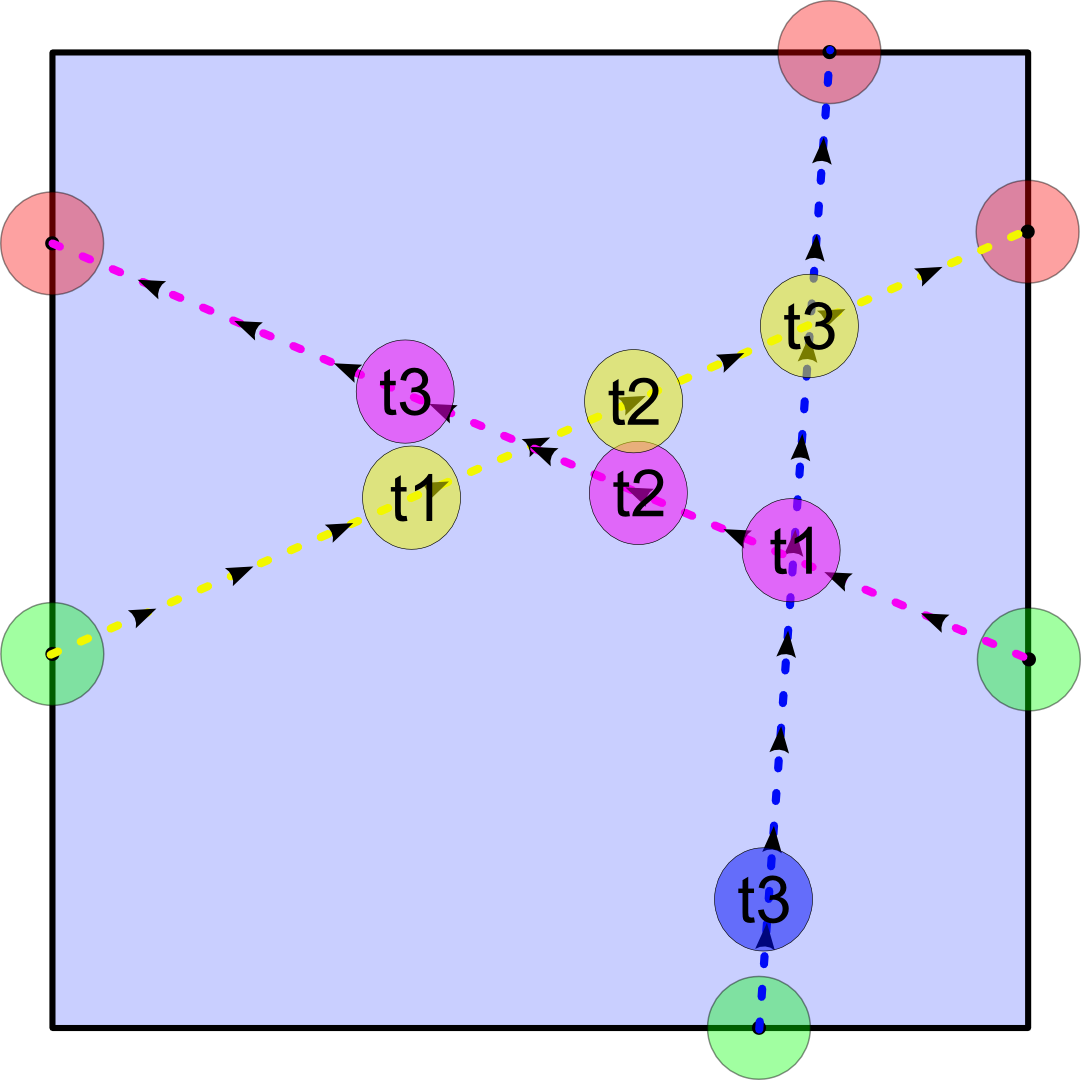
\includegraphics[width=0.3\linewidth]{./images/collision-2D-example-with-collision.png}
	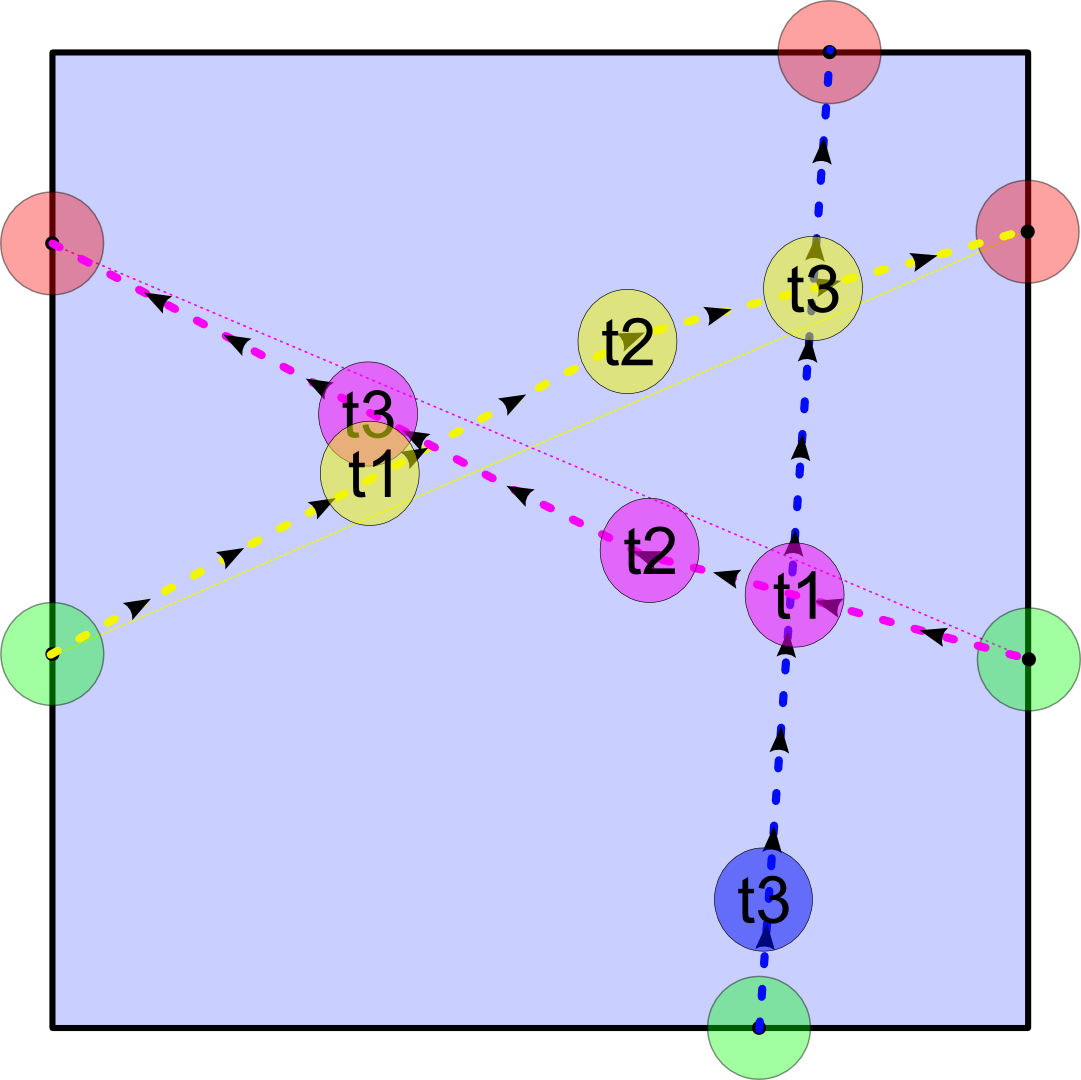
\includegraphics[width=0.3\linewidth]{./images/collision-2D-example-without-collision.png}
	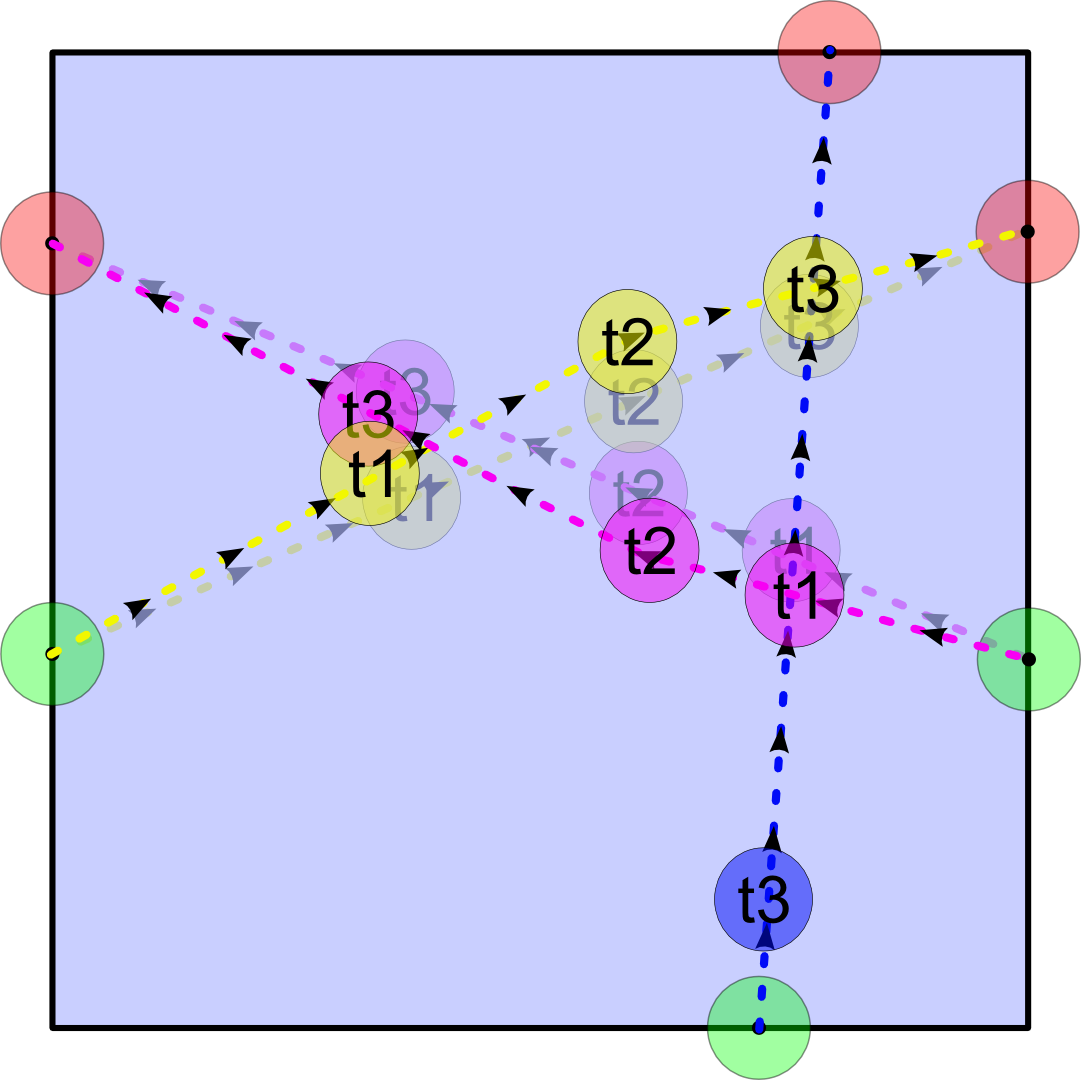
\includegraphics[width=0.3\linewidth]{./images/collision-2D-example-overlay.png}
	\\
	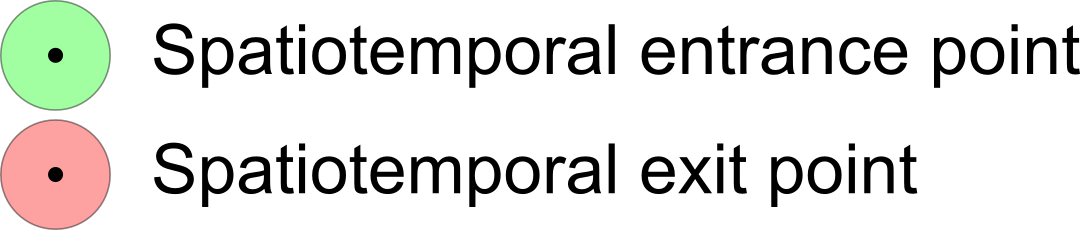
\includegraphics[width=0.3\linewidth]{./images/key-entry-exit-point.png}
	\caption{
		\textbf{\textbf{Collision removal}}
	}
	\label{fig:collision-removal}
	\end{center}
\end{figure*}
%%-------------------------------------------------------------------
%% Removing collisions figure
%%-------------------------------------------------------------------




We compute a minimum distance between each pair of trajectories. We store each value in a minimum distance matrix $M$. The position in the matrix corresponds to the trajectory ID. So the value at $M(i, j)$ would be the minimum distance from trajectory $\tau_i$ to trajectory $\tau_j$. It's good to note that this value will be the same as $M(j,i)$. Furthermore $M(i,i)$ will always be zero and distance for trajectories that don't intersect in time, we set them to a number bigger than the threshold for collisions, for example $100$ for a threshold of $1$ (see Table ~\ref{tab:minimum-distances}). These facts can be used to reduce computation while filling out the minimum distance matrix.

%%-------------------------------------------------------------------
%% The Minimum Distances Table
%%-------------------------------------------------------------------
\begin{table}[t]
	\centering
	\caption{Minimum Distances}
	\begin{tabular}{|c||c|c|c|}
		\hline
		 & $\tau_0$	& $\tau_1$ & $\tau_2$\\ \hline \hline
		$\tau_0$	& $0$		&	$100$ & $8.31$\\  \hline
		$\tau_1$	& $100$		&	$0$ & $0.14$\\  \hline
		$\tau_2$	& $8.31$		&	$0.14$ & $0$\\
		\hline
		\end{tabular}
\label{tab:minimum-distances}
\end{table}
%%-------------------------------------------------------------------
%% The Proposal List table
%%-------------------------------------------------------------------

\panayiotis{Do we have an image for this distance matrix?}
\memo{Actual image? Or a table? I can do that anyways, as soon as I figure out how to create a nxn table in latex}

Our algorithm (see Algorithm~\ref{algo:control-points}) creates collision free trajectories by adding and modifying control points. We can guarantee this by looking at the minimum distance matrix. If every value in the matrix is above some threshold then we know that for the entire period of the patch no two agents come closer than that threshold. So if we make that threshold equal to the sum of the radii being compared, those agents will never touch.

\panayiotis{Write the pseudo code in an algorithm format}

%%-------------------------------------------------------------------
%% Control Points algorithm
%%-------------------------------------------------------------------
\begin{algorithm}[t]
Compute minimum distance matrix $M$\;
\While{there exists at least one entry in $M$ below the threshold}{
	Find indices $i$  and $j$ for which $M(i,j)$ has the smallest value $d$\;
	Create temporary control points $\mathbf{cp}_i$ and $\mathbf{cp}_j$ in $\tau_i$ and $\tau_j$ that are at distance $d$ \;
	Apply repulsion forces to $\mathbf{cp}_i$ and $\mathbf{cp}_j$\;
	Update  $\tau_i$ and $\tau_j$\;
	Update $M$ \;
	}
\caption{The control points generation algorithm}
\label{algo:control-points}
\end{algorithm}
%%-------------------------------------------------------------------
%% Control Points algorithm
%%-------------------------------------------------------------------


We begin by computing the minimum distance matrix. Then while collisions still exist we find the smallest value in the minimum distance matrix. From that we find the corresponding trajectories and a point of closest approach for each trajectory $\mathbf{p}_1$ and $\mathbf{p}_2$. We then find an updated position for each of these points.

To find the the updated position of a new point we add a correction force $\mathbf{F}_c$ to its current position $\mathbf{p}_1^{old}$.


\begin{equation}
	\mathbf{p}_1^{new} = \mathbf{p}_1^{old} + \mathbf{F}_{c_1}
\end{equation}

\panayiotis{Why $P_1$ and not just $\mathbf{p}$? Clarify p1 and p2}

\panayiotis{assign symbols for all forces and position mentioned to make the equations more compact\ldots}

The correction force $\mathbf{F}_c$ for each point is found based on: the radius of the two agents, $r_1$ and $r_2$, which define a threshold $e=r_1+r_2$; a constant weight to help reduce speed artifacts and prevent agents from leaving the bounds the patch $w_1$ and $w_2$, each of them depending on the values of speeds $u_1$ and $u_2$; and a small random noise rotation matrix $R$ to help prevent infinite loops, the angle of rotation is chosen between $-.5$ and $.5$ radians.

\begin{equation}
	 \mathbf{F}_{c_1}= R  \widehat{(\mathbf{p}_1 - \mathbf{p}_2)}* e * w_1
\end{equation}
\memo{Do we need the wide hat?}

NOTE: In our implementation $r_1 = r_2$, making the threshold constant.

\panayiotis{SHORTEN THE TEXT IN THE EQUATIONS!!}
\begin{equation}
w_1 = \left\{
	\begin{array}{l l}
		u_2 / (u_1 + u_2)	&	\quad \text{if the point won't go outside the patch.}\\
		0								&	\quad \text{otherwise}
	\end{array}
	\right.
\end{equation}

The calculations for $\mathbf{p}_2$ are symmetric. Once we have this new point for the trajectory we check to see if there is already a control point within a small time interval of the new point. If there is we move that control point to this new position in space and time. Otherwise we add a control 
point in the trajectory at this new position. Finally we update the minimum distance matrix. We do not need to recheck all the distances in the matrix, only the ones that interact with the trajectory we have modified.

We find that in many situations this algorithm converges quickly and produces collision free trajectories. However there are still situations where it converges slowly or even gets stuck in an infinite loop.

\subsection{Smoothing}
\label{sec:method:smoothing}

Smoothing:
We have obtained some collision free trajectories, but they may have a jerky trajectory, so we need a final the step to smooth them. We need to take special care of how we do this, we donӴ want the trajectories to change in such a way that they make new collisions. A simple approach is to use cubic splines. Cubic splines connects every pair of points in a trajectory with a polynomial function of degree $3$:

\begin{equation}
 S(x)=a+bx+ cx^2+ dx^3
\end{equation}

In total, we will need to find the coefficients a, b, c, and d for every segment we have in our trajectory. Those coefficients are determined by continuity $C^1$ restrictions: 

For every spline associated with a trajectory between control point $\mathbf{cp}_1=(\mathbf{p}_1,t_1)$ and $\mathbf{cp}_2=(\mathbf{p}_2,t_2)$, the spline must pass through those same points, that is, $S(t_1)=(\mathbf{p}_1)$ and $S(t_2)=(\mathbf{p}_2)$.

For every two contiguous splines $S_1$ and $S_2$, for the common point they share p, the velocity must be equivalent, that is,  $S'_1(\mathbf{p})=S'_2Ҩ\mathbf{p})$.
  
This restrictions can be accommodated in a such way that they form a system of linear equations that can be solved using Cholesky decomposition.

We can not apply directly this method using our current control points. That results in trajectories that vary too much from the original, thus they may end up creating new collisions. To make the spline more similar to the original trajectory, we add new virtual control points sampled uniformly in the linear segments of the trajectories. We call these tacks. These tacks help fix the splines, because they will now pass through the control points and the tacks. Note that the more tacks we put, the closer the spline will fit to the original path.

After that, we compute the coefficients to create the splines and resample along the spline to get new control points. The new trajectory will still be composed of line segments, but since they are smaller, and following closely the path of a cubic function, to the naked eye they will look like curves. The finer the sample, the more it will look like a smooth path.

For optimization purposes, the second sampling is not taken uniformly. The trajectories are relatively straight in the middle of the the segments and have higher curvature near control points. For that reason, we take more samples around inflexion points (old control points) than far from them. These samples become the new control points that define the trajectory.

There may be cases, even with a healthy number of tacks, that the splines still vary too much from the original trajectory. We define a threshold based on the same threshold of collision to know how far a way a point can be moved. For these cases where the new control point surpasses the threshold, we simply donӴ add it to the set of new control points.  There may be extreme cases (for example, due to too a bad sampling of the tacks at the beginning), where the spline has extreme curves that are very different from our initial trajectory. In those extreme cases most of the new control points would not be added and the new smooth trajectory would end up being very similar to the original one.

Having splines for trajectories is better than having simple straight lines, but we know humans donӴ  follow either of them when walking,  so other methods can be tried to improve this initial approach.


